 
 The previous chapters detailed the proposed methodology for network inference from incomplete abundance data. The species abundances $\Ybf$ are jointly modeled in a GLMM using the Poisson log-normal distribution, thus taking advantage of its properties to account for offsets and experimental and/or environmental covariates $\Xbf$. The problem of network inference is then transposed to the Gaussian latent layer of model parameters $\Zbf$, where it is performed using averaging on spanning-tree structures with decomposable distribution on trees parametrized with edges weights $\betabf$. Missing actors are inferred in the Gaussian layer as well, simultaneously with the network. We remind the mathematical writing of this model:
  \begin{equation*}
 \left\{ \begin{array}{l}
 \begin{array}{ll}
 T\sim \prod_{kl\in T} \beta_{kl} / B, &B= \sum_{T\in\mathcal{T}} \prod_{kl \in T} \beta_{kl},\\\\
 \Zbf_i\mid T  \sim \Ncal (0, \Omegab_T), &\{\Zbf_i\}_i \text{ iid, }\\
 \end{array} \\\\
 Y_{ij}\mid \Zbf_i\sim \Pcal (\exp (o_{ij}+\xb_i^\intercal \thetab_j + Z_{ij})), \; (Y_{ij} \independent) \mid \Zbf_i 
 \end{array} \right.
 \end{equation*}
 
 The qualities of this approach have been demonstrated on simulated examples as well as empirical datasets. But why does it work ? Mostly because exact computations are possible in the Gaussian layer, thanks to its maniability and the structure and algebraic properties of spanning trees.  This flexibility calls for some natural extensions which were not developed due to time constraints, that we now present together with specific details of this approach.
 
 
\section{Sensitive details}
The presented methodology allows to take into account covariates and offsets, which is paramount in the modeling of experiments. A change in the covariates included can greatly modify the inferred network, however this is an information that can be controlled. On the other hand, not including offsets amounts to model incoherent data and therefore yields uninterpretable results. Unfortunately, offsets are not always obvious or easy to get, and evaluating them possibly represents a modeling step in itself. For example in an ecological census of fauna, the offset has to at least account for the period of time of observation, the experience of the observer and the species detectability, which is obviously the most difficult to get. Detectability depends on the relative position of the species to the observer, and can depend on the environmental conditions as well, making its modeling a delicate step.\\

The approach can also infer missing actors as detailed in Chapter 3. The initialization of the algorithm for this inference requires an initial clique of neighbors for each missing actor. This parameter is critical, as it defines all the initialization and if it is too far from the true clique, that is if not a minimum of true neighbors are included, the procedure can degenerate and abort. Several methods for setting this parameter are proposed in the \texttt{nestor} package. They are based on finding groups of highly correlated variables (sparse PCA and model-based clustering of the estimated correlation matrix), or finding clusters in the structure of the marginal graph (using Stochastic Bloc Models). The estimated lower bound of the likelihood can be used to choose between a large set of results with different initializations, thus one way to go is simply to sample several starting points (possibly by boostrapping the previous methods) and test all of them. Many other methods could be used, as well as prior knowledge on species, and we do not conclude on the best way to initialize the cliques. However we observed that it is less important for the inference quality to be precise than to include some true neighbors in the clique. Therefore we advise to choose the initial clique also based on its dimension.\\

One key question when working with possibly incomplete data is to know if it is indeed incomplete, and to what extend. This amounts to model selection to chose the number of missing actors $r$.  Usually model selection is carried out with computations on the likelihood of each model. As the model we developed involves several latent parameters, the inference is performed in a variational framework, yielding a lower bound of the likelihood. Moreover as we take advantage of the variational estimation of the PLNmodel described in \citet{CMR18}, we actually compute an approximation of this lower bound. This results in the usual model selection tools to not work (Akaike/Bayesian/Extended Bayesian Information Criterion). Model selection for models with variational inference is actually still an open research question of statistical theory.
 
\section{Extensions of the adopted approach}
In this section, we show direct extensions of the developed methodology regarding the network in itself (estimation of its parameters, network comparison), and the data nature (processing of different data types and spatialized data).
\subsection{Characterizing species interactions}


Generally, species interactions are characterized by their sign and strength. This information is contained in  the partial correlation matrix which is simply the opposite of the correlation matrix build from $\Omegabf$. Some methods are thus dedicated to the estimation of the partial correlation matrix to build knowledge on an ecosystem functioning. In the context of Gaussian Graphical Models, \cite{Lau96} develop maximum likelihood estimators for the precision matrix which depends on that of the covariance matrix, and the structure of the graph, as detailed in section \ref{ggm:mle}. It thus requires the precise knowledge of the graph, and even more than that: the only terms of the covariance matrix that are correctly estimated are those corresponding to edges in the graph. Therefore the prior inference of the structure is necessary. Moreover, these MLE are only valid for decomposable graph. Therefore following these three steps: 
\begin{enumerate}
\item Infer the conditional dependency structure $\G$,
\item Make $\G$ a chordal graph,
\item Compute $\widehat{\Omegabf}_{MLE}$
\end{enumerate}
 would lead to an approximation of $\Omegabf$. If the inferred network is already chordal, this would yield a proxy to the MLE of $\Omegabf$, available after the network inference.


\subsection{Network comparison}
 
Comparing networks has many applications and  yields results of interest in various fields, regarding for example the evolution of a system across seasons, or how a pathogen modifies the organization of a microbiome.
%comparison of embeddings ?
The comparison from a statistical point of view is linked to testing differences, or questioning the independence of two networks for example.  Rather than defining statistical tests based on networks distributions, current strategies consists in summarizing networks with measures, or vectors of measures, called embeddings. The latter can then be compared using PCA for example.
The presented approach assumes the graph is a latent tree, which distribution is estimated and can be seen as another available embedding. A first step toward statistical network comparison using trees could be to compare the estimated laws on trees, for example using the Küllback-Leibler divergence.

We denote $p_{\betabf_{\setminus kl}}$ the  decomposable tree distribution where the weight $\beta_{kl}$ is set to zero. Computing the Küllback-Leibler divergence between $p_\betabf$ and $p_{\betabf_{\setminus kl}}$ yields  the contribution of an edge to  the tree distribution. It writes:
\begin{align*}
KL(p_{\betabf_{\setminus kl}} (T) \mid\mid p_\betabf (T)) &= -\Esp_{p_\betabf (T)} [\log p_\betabf (T) - \log p_{\betabf_{\setminus kl}} (T)]\\
&=P_{kl} \log \beta_{kl} + \log ( B_{\setminus kl}/B)\\
&=P_{kl} \log \beta_{kl} + \log (1-P_{kl})
\end{align*}

%peut être utile pour ordonner les arêtes par importance si trop de probabilités égales. Besoin de faire un test pour voir si la qté existe 	vec une proba à 1 (existance de B\kl)
As the distribution under which the expectation is taken must be dominant over the other, the divergence $KL(p_\betabf (T)\mid\mid p_{\betabf_{\setminus kl}} (T)) $ is not defined.

If all edges weights are finite and non-nulls, the divergence can be symmetrized into a dissymetry measure. Considering two weight matrices $\betabf^A$ and $\betabf^B$, the dissymetry between the tree distributions they define is
\begin{align*}
D(p_{\betabf^A}, p_{\betabf^B}) &=\frac{1}{2} \left[KL\big( p_{\betabf^B} (T) \mid\mid p_{\betabf^A}(T)\big)+KL\big( p_{\betabf^A}(T)\mid\mid p_{\betabf^B} (T)  \big)\right]\\
&=\sum_{kl} ( P_{kl}^A - P_{kl}^B) ) \big(\log \betabf^B - \log \betabf^A\big)
\end{align*}

where $P_{kl}^A = \Esp_{p_{\betabf^A}}[\mathds{1}\{kl\in T\}]$


%(si temps pour exemple, MDS 2 premiers axes)

\subsection{Data types}
This work focuses on abundance data, however the network inference method developed here could be extended to other data types. Indeed, the strategy of tree averaging is based on the Gaussian Layer of the $\Zbf$. Therefore it could also be used with a model which would keep this layer and add a different emission law than the Poisson to generate data $\Ybf$.

For example, choosing another emission law could yield presence/absence data (binomial distribution), ordinal data (multinomial distribution) or positive continuous data to model biomass (tweedie distribution). Mixed data could also be generated, as long as the emission law parameters are stored in a Gaussian layer. 

Another interesting extension of the emission law is for it to generate multidimensional data.  In the case of counts, this is known as multi-attribute counts. Nodes of the network would then represent vectors of information (e.g. \textcolor{red}{example, and edges})

For all these examples, the mechanic of network inference in the Gaussian layer would remain the same. The only step left would be to estimate the emission law parameters.


\subsection{Spatial dependence}
In ecological surveys, environmental conditions might be spatially heterogeneous (e.g. different climate at different altitudes).   This translates in spatial correlation in the observed data, which has to be accounted for in the network inference.

Spatial correlation is due to spatially close environments being similar. Therefore a first and quick way to correct for spatial dependence is to include spatial covariates in the model. For example Figure \ref{vario} shows how a variogram may be flattened by adjusting for spatial coordinates.
\begin{figure}
\centering
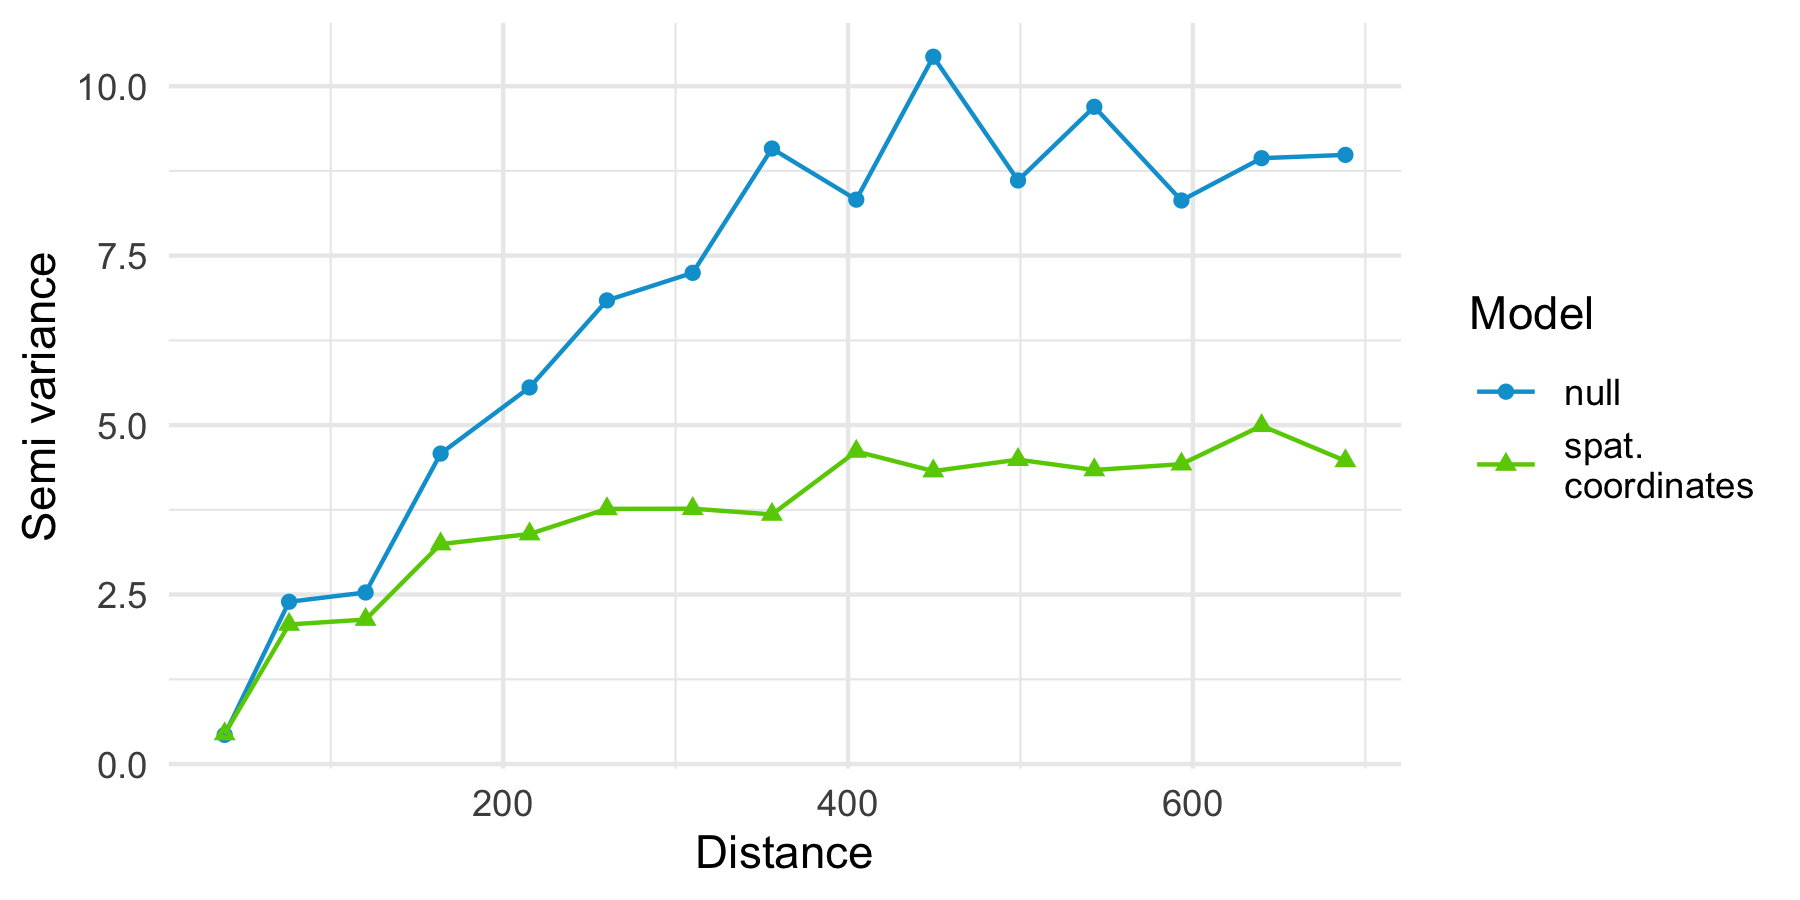
\includegraphics[width=10cm]{figs/variogram.png}
\caption{Variogram of the species Trisopterus esmarkii (Norway pout) from the Barents dataset with and without adjusting linearly for the spatial coordinates.}
\label{vario}
\end{figure}
However such correction might not be enough and the residuals might still be spatially correlated. Spatial coordinates could be adjusted in a more complicated way than the linear relationship, but another solution is to consider this dependence to be the result of an unobserved variable. As a missing variable, the spatial dependence can be taken into account to unravel the dependencies of interest by using the method detailed in Chapter 3.

These two solutions aim at correcting for the spatial effect, which is thus considered as a kind of noise on the signal of species dependencies. However, one might be interested in modeling this spatial effect for further study. In that case, a first approach is to assume a separation of the dependencies due to the spatial effects ($\Delta$) on the one hand, and due to the species interactions ($\Sigma$) on the other hand. This means that dependencies are studied between several species in the same sampling site, or between several sampling sites for the same species, and that independence is assumed between different species at different sites. It would then be possible to write a pairwise composite log-likelihood of count data $\Ybf$ as follows:
$$c\ell_\theta(\Ybf) = \sum_{j=1}^p \sum_{s<t} \log p_\theta(Y_{sj}, Y_{tj})+\sum_{s=1}^n \sum_{j<k} \log p_\theta(Y_{sj}, Y_{sj})$$
% en utilisant les arbres ? les lois bivariées suffisent
%reste vraisemblance composite, poilog bivarié, pourquoi 2 par 2 en fait

 %In the context of counts modeled with a Gaussian latent layer, this leads to the modeling of the variance-covariance matrix $\Gamma$ of the Gaussian layer as the Kronecker product between the two dependencies: $\Gamma = \Delta \otimes \Sigma$. 
 
%ovaskainen hmsc fait le job, à vérifier

\section{Network inference in the observed layer}
All of the above is an adaptation of the presented model to perform network inference in the latent Gaussian layer of parameters. However it has been demonstrated that if the latent network is connex, then the grpahical model on the counts $\Ybf$ is simply a clique. \textcolor{red}{ref}. The primary goal is to infer the network directly from $\Ybf$, without resorting to a Gaussian space.

\begin{itemize}
\item motivation
\item écriture des modèles par arbres, distribution conditionnelle à l'arbre proportionnelle au produit sur les arêtes, moyenne d'arbres
\item la loi bivariée suffit, parler faithfulness avec bipoilog 5 paramètres paramètre de dépendance
\item  l'estimation peut être mega dure
\end{itemize}
